% Template adapted from https://github.com/jgm/pandoc-templates/blob/master/default.latex
% To be used with XeLaTex in memoiR
%%%%%%%%%%%%%%%%%%%%%%%%%%%%%%%%%%%%%%%%%%%%%%%%%%%%%%%%%%%%%%%%%%%%%%%%%%%%%%%%%%%%%%%%%

% Options for packages loaded elsewhere
\PassOptionsToPackage{unicode=true}{hyperref}
\PassOptionsToPackage{hyphens}{url}
\PassOptionsToPackage{dvipsnames,svgnames*,x11names*}{xcolor}
% Right to left support


\documentclass[
  10pt,
  italian,
  a4paper,
  extrafontsizes,onecolumn,openright
  ]{memoir}

% Double (or whatever) spacing

% Math
\usepackage{amssymb, amsmath}
% mathspec: arbitrary math fonts
\usepackage{unicode-math}
\defaultfontfeatures{Scale=MatchLowercase}
\defaultfontfeatures[\rmfamily]{Ligatures=TeX,Scale=1}

% Fonts
\usepackage{lmodern}
\usepackage{fontspec}

% Main font
% Specific sanserif font
% Specific monotype font
\setmonofont[Scale=0.75]{Operator Mono SSm Lig Book}
% Specific math font
% Chinese, Japanese, Corean fonts

% Use upquote for straight quotes in verbatim environments
\usepackage{upquote}
% Use microtype
\usepackage[]{microtype}
\UseMicrotypeSet[protrusion]{basicmath} % disable protrusion for tt fonts

% Verbatim in note

% Color links
\usepackage{xcolor}

% Strikeout

% Necessary for code chunks
\usepackage{color}
\usepackage{fancyvrb}
\newcommand{\VerbBar}{|}
\newcommand{\VERB}{\Verb[commandchars=\\\{\}]}
\DefineVerbatimEnvironment{Highlighting}{Verbatim}{commandchars=\\\{\}}
% Add ',fontsize=\small' for more characters per line
\usepackage{framed}
\definecolor{shadecolor}{RGB}{248,248,248}
\newenvironment{Shaded}{\begin{snugshade}}{\end{snugshade}}
\newcommand{\AlertTok}[1]{\textcolor[rgb]{0.94,0.16,0.16}{#1}}
\newcommand{\AnnotationTok}[1]{\textcolor[rgb]{0.56,0.35,0.01}{\textbf{\textit{#1}}}}
\newcommand{\AttributeTok}[1]{\textcolor[rgb]{0.77,0.63,0.00}{#1}}
\newcommand{\BaseNTok}[1]{\textcolor[rgb]{0.00,0.00,0.81}{#1}}
\newcommand{\BuiltInTok}[1]{#1}
\newcommand{\CharTok}[1]{\textcolor[rgb]{0.31,0.60,0.02}{#1}}
\newcommand{\CommentTok}[1]{\textcolor[rgb]{0.56,0.35,0.01}{\textit{#1}}}
\newcommand{\CommentVarTok}[1]{\textcolor[rgb]{0.56,0.35,0.01}{\textbf{\textit{#1}}}}
\newcommand{\ConstantTok}[1]{\textcolor[rgb]{0.00,0.00,0.00}{#1}}
\newcommand{\ControlFlowTok}[1]{\textcolor[rgb]{0.13,0.29,0.53}{\textbf{#1}}}
\newcommand{\DataTypeTok}[1]{\textcolor[rgb]{0.13,0.29,0.53}{#1}}
\newcommand{\DecValTok}[1]{\textcolor[rgb]{0.00,0.00,0.81}{#1}}
\newcommand{\DocumentationTok}[1]{\textcolor[rgb]{0.56,0.35,0.01}{\textbf{\textit{#1}}}}
\newcommand{\ErrorTok}[1]{\textcolor[rgb]{0.64,0.00,0.00}{\textbf{#1}}}
\newcommand{\ExtensionTok}[1]{#1}
\newcommand{\FloatTok}[1]{\textcolor[rgb]{0.00,0.00,0.81}{#1}}
\newcommand{\FunctionTok}[1]{\textcolor[rgb]{0.00,0.00,0.00}{#1}}
\newcommand{\ImportTok}[1]{#1}
\newcommand{\InformationTok}[1]{\textcolor[rgb]{0.56,0.35,0.01}{\textbf{\textit{#1}}}}
\newcommand{\KeywordTok}[1]{\textcolor[rgb]{0.13,0.29,0.53}{\textbf{#1}}}
\newcommand{\NormalTok}[1]{#1}
\newcommand{\OperatorTok}[1]{\textcolor[rgb]{0.81,0.36,0.00}{\textbf{#1}}}
\newcommand{\OtherTok}[1]{\textcolor[rgb]{0.56,0.35,0.01}{#1}}
\newcommand{\PreprocessorTok}[1]{\textcolor[rgb]{0.56,0.35,0.01}{\textit{#1}}}
\newcommand{\RegionMarkerTok}[1]{#1}
\newcommand{\SpecialCharTok}[1]{\textcolor[rgb]{0.00,0.00,0.00}{#1}}
\newcommand{\SpecialStringTok}[1]{\textcolor[rgb]{0.31,0.60,0.02}{#1}}
\newcommand{\StringTok}[1]{\textcolor[rgb]{0.31,0.60,0.02}{#1}}
\newcommand{\VariableTok}[1]{\textcolor[rgb]{0.00,0.00,0.00}{#1}}
\newcommand{\VerbatimStringTok}[1]{\textcolor[rgb]{0.31,0.60,0.02}{#1}}
\newcommand{\WarningTok}[1]{\textcolor[rgb]{0.56,0.35,0.01}{\textbf{\textit{#1}}}}

% Listings package

% Tables
\usepackage{longtable,booktabs,tabu}
% Fix footnotes in tables (requires footnote package)
\IfFileExists{footnote.sty}{\usepackage{footnote}\makesavenoteenv{longtable}}{}

% Graphics
\usepackage{graphicx,grffile}
\graphicspath{{images/}}
\makeatletter
\def\maxwidth{\ifdim\Gin@nat@width>\linewidth\linewidth\else\Gin@nat@width\fi}
\def\maxheight{\ifdim\Gin@nat@height>\textheight\textheight\else\Gin@nat@height\fi}
\makeatother
% Scale images if necessary, so that they will not overflow the page
% margins by default, and it is still possible to overwrite the defaults
% using explicit options in \includegraphics[width, height, ...]{}
\setkeys{Gin}{width=\maxwidth,height=\maxheight,keepaspectratio}

% Prevent overfull lines
\setlength{\emergencystretch}{3em}  
\providecommand{\tightlist}{%
  \setlength{\itemsep}{0pt}\setlength{\parskip}{0pt}}

% Number sections for memoir (secnumdepth counter is ignored)
\setsecnumdepth{section}

% Set default figure placement to htbp
\makeatletter
\def\fps@figure{htbp}
\makeatother

% Spacing in lists
\usepackage{enumitem}

% Polyglossia
\usepackage{polyglossia}
\setmainlanguage{it}
\setotherlanguage{en-US}

% BibLaTeX
\usepackage[backend=biber,style=authoryear-ibid,isbn=false,backref=true,giveninits=true,uniquename=init,maxcitenames=2,maxbibnames=150,sorting=nyt,sortcites=false,style=apa]{biblatex}
\addbibresource{refs.bib}

% cslreferences environment required by pandoc > 2.7



%%%%%%%%%%%%%%%%%%%%%%%%%%%%%%%%%%%%%%%%%%%%%%%%%%%%%%%%%%
% memoiR format

% Chapter Summary environment 
\usepackage[tikz]{bclogo}
\newenvironment{Summary}
  {\begin{bclogo}[logo=\bctrombone, noborder=true, couleur=lightgray!50]{In breve}\parindent0pt}
  {\end{bclogo}}
% Syntax:
%
%```{block, type='Summary'}
% Deliver message here.
% ```

% scriptsize code 
\let\oldverbatim\verbatim
\def\verbatim{\oldverbatim\scriptsize}
% Applies to code blocks and R code results
% code chunk options size='scriptsize' applies only to R code and results
% if the code chunk sets a different size, \def\verbatim{...} is prioritary for code results 


% Layout
%%%%%%%%%%%%%%%%%%%%%%%%%%%%%%%%%%%%%%%%%%%%%%%%%%%%%%%%%%

% Based on memoir, style companion
\newcommand{\MemoirChapStyle}{daleif1}
\newcommand{\MemoirPageStyle}{Ruled}

% Space between paragraphs
\usepackage{parskip}
  \abnormalparskip{3pt}

% Adjust margin paragraphs vertical position
\usepackage{marginfix}


% Margins
%%%%%%%%%%%%%%%%%%%%%%%%%%%%%%%%%%%%%%%

% allow use of '-',+','/' ans '*' to make simple length computation
\usepackage{calc}

% Full-width figures utilities
\newlength\widthw % full width
\newlength{\rf}
\newcommand*{\definesHSpace}{
  \strictpagecheck % slower but efficient detection of odd/even pages
  \checkoddpage
  \ifoddpage
  \setlength{\rf}{0mm}
  \else
  \setlength{\rf}{\marginparsep+\marginparwidth}
  \fi
}

\makeatletter
% 1" margins for the front matter.
\newcommand*{\SmallMargins}{
  \setlrmarginsandblock{1.5in}{1.5in}{*}
  \setmarginnotes{0.1in}{0.1in}{0.1in}
 \setulmarginsandblock{1.5in}{1in}{*}
  \checkandfixthelayout
  \ch@ngetext
  \clearpage
  \setlength{\widthw}{\textwidth+\marginparsep+\marginparwidth}
  \footnotesatfoot
  \chapterstyle{\MemoirChapStyle}  % Chapter and page styles must be recalled
  \pagestyle{\MemoirPageStyle}
}

% 3" outer margin for the main matter
\newcommand{\LargeMargins}{\SmallMargins}
\makeatother

% Figure captions and footnotes in outer margins


% Main title page with filigrane
%%%%%%%%%%%%%%%%%%%%%%%%%%%%%%%%%%%%%%%%%%%%%%%%%%%%%%%%%%

% Text blocks
\usepackage[absolute,overlay]{textpos}
  \setlength{\TPHorizModule}{1mm}
  \setlength{\TPVertModule}{1mm}

\newcommand{\MainTitlePage}[2]{
  \SmallMargins % Margins
  \pagestyle{empty} % No header/footer
  \textblockorigin{\stockwidth-\paperwidth-\trimedge}{\trimtop} % recto
  \begin{textblock*}{2mm}(\spinemargin/2,\uppermargin/2)
    \rule{1pt}{\paperheight-\uppermargin}
  \end{textblock*}
  \begin{textblock*}{\paperwidth*2/3}(\paperwidth/5, \paperheight/5)
    \flushright
    \begin{Spacing}{3}
      {\fontfamily{qtm}\selectfont\fontsize{45}{45}\selectfont\textsc{\thetitle}}
    \end{Spacing}
  \end{textblock*}
    \begin{textblock*}{\paperwidth*2/3}(\paperwidth/5, \paperheight/2)
    \flushright
    {\fontfamily{qtm}\huge\theauthor}
  \end{textblock*}
    \begin{textblock*}{\paperwidth*2/3}[0, 1](\spinemargin, \uppermargin+\textheight)
    \normalfont\thedate
  \end{textblock*}
  ~\\ % Print a character or the page will not exist
  \newpage
  \textblockorigin{\trimedge}{\trimtop} % verso
  \begin{textblock*}{\textwidth}(\paperwidth-\spinemargin-\textwidth, \uppermargin)
    #1
  \end{textblock*}
  \begin{textblock*}{\textwidth}[0,1](\paperwidth-\spinemargin-\textwidth, \uppermargin+\textheight+\footskip)
    \centering
    
\includegraphics[width=\paperwidth/4]{logo}\\ \bigskip
    #2
  \end{textblock*}
  ~\\ % Print a character or the page will not exist
  \newpage
}

% Clear page and open an even one (\clearpage opens an odd one)
\newcommand{\evenpage}{
  \clearpage
  \strictpagecheck % slower but efficient detection of odd/even pages
  \checkoddpage
  \ifoddpage
    \thispagestyle{empty}
    ~\\ % Print a character or the page will not exist
    \newpage
  \else
    % do nothing
  \fi
}


%% PDF title page to insert
%%%%%%%%%%%%%%%%%%%%%%%%%%%%%%%%%%%%%%%%%%%%%%%%%%%%%%%%%%



%% Bibliography
%%%%%%%%%%%%%%%%%%%%%%%%%%%%%%%%%%%%%%%%%%%%%%%%%%%%%%%%%%

\usepackage[strict,autostyle]{csquotes}
% Repeated citation as author-year-title instead of author-title (modification of footcite:note in verbose-inote.cbx)

%% Table of Contents
%%%%%%%%%%%%%%%%%%%%%%%%%%%%%%%%%%%%%%%%%%%%%%%%%%%%%%%%%%

% fix the typesetting of the part number
\renewcommand\partnumberlinebox[2]{#2\ ---\ }


% Fonts
%%%%%%%%%%%%%%%%%%%%%%%%%%%%%%%%%%%%%%%%%%%%%%%%%%%%%%%%%%


% Hyperref comes last
%%%%%%%%%%%%%%%%%%%%%%%%%%%%%%%%%%%%%%%%%%%%%%%%%%%%%%%%%%

\usepackage{hyperref}
\hypersetup{
  pdftitle={Psicometria},
  pdfauthor={Corrado Caudek},
  colorlinks=true,
  linkcolor=Maroon,
  citecolor=Blue,
  urlcolor=Blue,
  breaklinks=true}

% Don't use monospace font for urls
\urlstyle{same}


% Title, author, date from YAML to LaTeX
%%%%%%%%%%%%%%%%%%%%%%%%%%%%%%%%%%%%%%%%%%%%%%%%%%%%%%%%%%

\title{Psicometria}

\author{Corrado Caudek}

\date{2021-11-30}


% Include headers (preamble.tex) here
%%%%%%%%%%%%%%%%%%%%%%%%%%%%%%%%%%%%%%%%%%%%%%%%%%%%%%%%%%
% Add LaTeX code into the preamble of the document here
\hyphenation{bio-di-ver-si-ty sap-lings}


%%%%%%%%%%%%%%%%%%%%%%%%%%%%%%%%%%%%%%%%%%%%%%%%%%%%%%%%%%%%%%%%%%%%%%%%%
% memoiR dalef3 chapter style 
% https://ctan.crest.fr/tex-archive/info/latex-samples/MemoirChapStyles/MemoirChapStyles.pdf
\usepackage{soul}
\definecolor{nicered}{rgb}{.647,.129,.149}
\makeatletter
\newlength\dlf@normtxtw
\setlength\dlf@normtxtw{\textwidth}
\def\myhelvetfont{\def\sfdefault{mdput}}
\newsavebox{\feline@chapter}
\newcommand\feline@chapter@marker[1][4cm]{%
  \sbox\feline@chapter{%
    \resizebox{!}{#1}{\fboxsep=1pt%
	  \colorbox{nicered}{\color{white}\bfseries\sffamily\thechapter}%
	}}%
  \rotatebox{90}{%
    \resizebox{%
	  \heightof{\usebox{\feline@chapter}}+\depthof{\usebox{\feline@chapter}}}%
	{!}{\scshape\so\@chapapp}}\quad%
  \raisebox{\depthof{\usebox{\feline@chapter}}}{\usebox{\feline@chapter}}%
 }
\newcommand\feline@chm[1][4cm]{%
  \sbox\feline@chapter{\feline@chapter@marker[#1]}%
  \makebox[0pt][l]{% aka \rlap
    \makebox[1cm][r]{\usebox\feline@chapter}%
  }}
\makechapterstyle{daleif1}{
  \renewcommand\chapnamefont{\normalfont\Large\scshape\raggedleft\so}
  \renewcommand\chaptitlefont{\normalfont\huge\bfseries\scshape\color{nicered}}
  \renewcommand\chapternamenum{}
  \renewcommand\printchaptername{}
  \renewcommand\printchapternum{\null\hfill\feline@chm[2.5cm]\par}
  \renewcommand\afterchapternum{\par\vskip\midchapskip}
  \renewcommand\printchaptertitle[1]{\chaptitlefont\raggedleft ##1\par}
}
\makeatother

\DeclareMathOperator{\Var}{Var} % Define variance operator
\DeclareMathOperator{\SD}{SD} % Define sd operator
\DeclareMathOperator{\Cov}{Cov} % Define covariance operator
\DeclareMathOperator{\Corr}{Corr} % Define correlation operator
\DeclareMathOperator{\Me}{Me} % Define mediane operator
\DeclareMathOperator{\Mo}{Mo} % Define mode operator
\DeclareMathOperator{\Bin}{Bin} % Define binomial operator
\DeclareMathOperator{\Bernoulli}{Bernoulli} % Define Bernoulli operator
\DeclareMathOperator{\Poi}{Poi} % Define Poisson operator
\DeclareMathOperator{\Uniform}{Uniform} % Define Uniform operator
\DeclareMathOperator{\Cauchy}{Cauchy} % Define Cauchy operator
\DeclareMathOperator{\elpd}{elpd} % Define elpd operator
\DeclareMathOperator{\lppd}{lppd} % Define lppd operator
\DeclareMathOperator{\LOO}{LOO} % Define LOO operator
\DeclareMathOperator{\B}{\mathscr{B}} % Define Bernoulli operator
\newcommand{\R}{\textsf{R}} % Define R programming language symbol
\newcommand{\E}{\mathbb{E}} % Define expected value operator
\newcommand{\Real}{\mathbb{R}} % Define real number operator
\newcommand{\Prob}{\mathscr{P}}
\DeclareMathOperator*{\argmin}{arg\,min} % thin space, limits on side in displays
\DeclareMathOperator*{\argmax}{arg\,max} % thin space, limits on side in displays

\raggedbottom % allow variable (ragged) site heights
\frenchspacing

\usepackage[
  labelfont=bf, 
  font={small, it} 
]{caption} 
\usepackage{upquote} % print correct quotes in verbatim-environments
\usepackage{empheq} 
\usepackage{xfrac}




\usepackage{booktabs}
\usepackage{longtable}
\usepackage{array}
\usepackage{multirow}
\usepackage{wrapfig}
\usepackage{float}
\usepackage{colortbl}
\usepackage{pdflscape}
\usepackage{tabu}
\usepackage{threeparttable}
\usepackage{threeparttablex}
\usepackage[normalem]{ulem}
\usepackage{makecell}
\usepackage{xcolor}


% End of preamble
%%%%%%%%%%%%%%%%%%%%%%%%%%%%%%%%%%%%%%%%%%%%%%%%%%%%%%%%%%


\begin{document}
\frontmatter

% Title page
%%%%%%%%%%%%%%%%%%%%%%%%%%%%%%%%%%%%%%%%%%%%%%%%%%%%%%%%%%


\MainTitlePage{Questo documento è stato realizzato con:

\begin{itemize}
  \item \LaTeX\; e la classe memoir (\url{http://www.ctan.org/pkg/memoir});
  \item $\R$ (\url{http://www.r-project.org/}) e RStudio (\url{http://www.rstudio.com/});
  \item bookdown (\url{http://bookdown.org/}) e memoiR (\url{https://ericmarcon.github.io/memoiR/}).
\end{itemize}}{Nel blog della mia pagina personale sono forniti alcuni approfondimenti degli argomenti qui trattati.

\url{https://ccaudek.github.io/caudeklab/}}


% Before Body
%%%%%%%%%%%%%%%%%%%%%%%%%%%%%%%%%%%%%%%%%%%%%%%%%%%%%%%%%%





% Contents
%%%%%%%%%%%%%%%%%%%%%%%%%%%%%%%%%%%%%%%%%%%%%%%%%%%%%%%%%%

\LargeMargins
{
\hypersetup{linkcolor=}
\setcounter{tocdepth}{2}
\tableofcontents
}


% Body
%%%%%%%%%%%%%%%%%%%%%%%%%%%%%%%%%%%%%%%%%%%%%%%%%%%%%%%%%%

\LargeMargins
\scriptsize

\normalsize

\chapter*{}

\vfill

\scriptsize

\normalsize

\scriptsize

Copyright \(\copyright\) 2022.

\normalsize

Data della versione presente: Novembre 30, 2021.

\hypertarget{prefazione}{%
\chapter{Prefazione}\label{prefazione}}

\textbf{Data Science per psicologi} contiene il materiale delle lezioni dell'insegnamento di \emph{Psicometria B000286} (A.A. 2021/2022) rivolto agli studenti del primo anno del Corso di Laurea in Scienze e Tecniche Psicologiche dell'Università degli Studi di Firenze.

L'insegnamento di Psicometria si propone di fornire agli studenti un'introduzione all'analisi dei dati in psicologia.
Le conoscenze/competenze che verranno sviluppate in questo insegnamento sono quelle della \emph{Data science}, ovvero le conoscenze/competenze che si pongono all'intersezione tra statistica (ovvero, richiedono la capacità di comprendere teoremi statistici) e informatica (ovvero, richiedono la capacità di sapere utilizzare un software).

\hypertarget{la-psicologia-e-la-data-science}{%
\section*{La psicologia e la Data Science}\label{la-psicologia-e-la-data-science}}
\addcontentsline{toc}{section}{La psicologia e la Data Science}

\begin{quote}
It's worth noting, before getting started, that this material is hard. If you find yourself confused at any point, you are normal. Any sense of confusion you feel is just your brain correctly calibrating to the subject matter. Over time, confusion is replaced by comprehension {[}\ldots{]} --- Richard McElreath
\end{quote}

Sembra sensato spendere due parole su un tema che è importante per gli studenti: quello indicato dal titolo di questo Capitolo. È ovvio che agli studenti di psicologia la statistica non piace. Se piacesse, forse studierebbero Data Science e non psicologia; ma non lo fanno. Di conseguenza, gli studenti di psicologia si chiedono: ``perché dobbiamo perdere tanto tempo a studiare queste cose quando in realtà quello che ci interessa è tutt'altro?'\,' Questa è una bella domanda.

C'è una ragione molto semplice che dovrebbe farci capire perché la Data Science è così importante per la psicologia. Infatti, a ben pensarci, la psicologia è una disciplina intrinsecamente statistica, se per statistica intendiamo quella disciplina che studia la variazione delle caratteristiche degli individui nella popolazione. La psicologia studia \emph{gli individui} ed è proprio la variabilità inter- e intra-individuale ciò che vogliamo descrivere e, in certi casi, predire. In questo senso, la psicologia è molto diversa dall'ingegneria, per esempio. Le proprietà di un determinato ponte sotto certe condizioni, ad esempio, sono molto simili a quelle di un altro ponte, sotto le medesime condizioni. Quindi, per un ingegnere la statistica è poco importante: le proprietà dei materiali sono unicamente dipendenti dalla loro composizione e restano costanti. Ma lo stesso non può dirsi degli individui: ogni individuo è unico e cambia nel tempo. E le variazioni tra gli individui, e di un individuo nel tempo, sono l'oggetto di studio proprio della psicologia: è dunque chiaro che i problemi che la psicologia si pone sono molto diversi da quelli affrontati, per esempio, dagli ingegneri. Questa è la ragione per cui abbiamo tanto bisogno della \emph{data science} in psicologia: perché la \emph{data science} ci consente di descrivere la variazione e il cambiamento. E queste sono appunto le caratteristiche di base dei fenomeni psicologici.

Sono sicuro che, leggendo queste righe, a molti studenti sarà venuta in mente la seguente domanda: perché non chiediamo a qualche esperto di fare il ``lavoro sporco'' (ovvero le analisi statistiche) per noi, mentre noi (gli psicologi) ci occupiamo solo di ciò che ci interessa, ovvero dei problemi psicologici slegati dai dettagli ``tecnici'' della \emph{data science}?
La risposta a questa domanda è che non è possibile progettare uno studio psicologico sensato senza avere almeno una comprensione rudimentale della \emph{data science}. Le tematiche della \emph{data science} non possono essere ignorate né dai ricercatori in psicologia né da coloro che svolgono la professione di psicologo al di fuori dell'Università. Infatti, anche i professionisti al di fuori dall'università non possono fare a meno di leggere la letteratura psicologica più recente: il continuo aggiornamento delle conoscenze è infatti richiesto dalla deontologia della professione. Ma per potere fare questo è necessario conoscere un bel po' di \emph{data science}! Basta aprire a caso una rivista specialistica di psicologia per rendersi conto di quanto ciò sia vero: gli articoli che riportano i risultati delle ricerche psicologiche sono zeppi di analisi statistiche e di modelli formali. E la comprensione della letteratura psicologica rappresenta un requisito minimo nel bagaglio professionale dello psicologo.

Le considerazioni precedenti cercano di chiarire il seguente punto: la \emph{data science} non è qualcosa da studiare a malincuore, in un singolo insegnamento universitario, per poi poterla tranquillamente dimenticare. Nel bene e nel male, gli psicologi usano gli strumenti della \emph{data science} in tantissimi ambiti della loro attività professionale: in particolare quando costruiscono, somministrano e interpretano i test psicometrici. È dunque chiaro che possedere delle solide basi di \emph{data science} è un tassello imprescindibile del bagaglio professionale dello psicologo. In questo insegnamento verrano trattati i temi base della \emph{data science} e verrà adottato un punto di vista bayesiano, che corrisponde all'approccio più recente e sempre più diffuso in psicologia.

\hypertarget{come-studiare}{%
\section*{Come studiare}\label{come-studiare}}
\addcontentsline{toc}{section}{Come studiare}

\begin{quote}
I know quite certainly that I myself have no special talent. Curiosity, obsession and dogged endurance, combined with self-criticism, have brought me to my ideas. --- Albert Einstein
\end{quote}

Il giusto metodo di studio per prepararsi all'esame di Psicometria è quello di seguire attivamente le lezioni, assimilare i concetti via via che essi vengono presentati e verificare in autonomia le procedure presentate a lezione. Incoraggio gli studenti a farmi domande per chiarire ciò che non è stato capito appieno. Incoraggio gli studenti a utilizzare i forum attivi su Moodle e, soprattutto, a svolgere gli esercizi proposti su Moodle. I problemi forniti su Moodle rappresentano il livello di difficoltà richiesto per superare l'esame e consentono allo studente di comprendere se le competenze sviluppate fino a quel punto sono sufficienti rispetto alle richieste dell'esame.

La prima fase dello studio, che è sicuramente individuale, è quella in cui è necessario acquisire le conoscenze teoriche relative ai problemi che saranno presentati all'esame. La seconda fase di studio, che può essere facilitata da scambi con altri e da incontri di gruppo, porta ad acquisire la capacità di applicare le conoscenze: è necessario capire come usare un software (\R) per applicare i concetti statistici alla specifica situazione del problema che si vuole risolvere. Le due fasi non sono però separate: il saper fare molto spesso ci aiuta a capire meglio.

\hypertarget{sviluppare-un-metodo-di-studio-efficace}{%
\section*{Sviluppare un metodo di studio efficace}\label{sviluppare-un-metodo-di-studio-efficace}}
\addcontentsline{toc}{section}{Sviluppare un metodo di studio efficace}

\begin{quote}
Memorization is not learning. --- Richard Phillips Feynman
\end{quote}

Avendo insegnato molte volte in passato un corso introduttivo di analisi dei dati ho notato nel corso degli anni che gli studenti con l'atteggiamento mentale che descriverò qui sotto generalmente ottengono ottimi risultati. Alcuni studenti sviluppano naturalmente questo approccio allo studio, ma altri hanno bisogno di fare uno sforzo per maturarlo. Fornisco qui sotto una breve descrizione del ``metodo di studio'\,' che, nella mia esperienza, è il più efficace per affrontare le richieste di questo insegnamento \autocite{burger20125}.

\begin{itemize}
\tightlist
\item
  Dedicate un tempo sufficiente al materiale di base, apparentemente facile; assicuratevi di averlo capito bene. Cercate le lacune nella vostra comprensione. Leggere presentazioni diverse dello stesso materiale (in libri o articoli diversi) può fornire nuove intuizioni.
\end{itemize}

\begin{itemize}
\item
  Gli errori che facciamo sono i nostri migliori maestri. Istintivamente cerchiamo di dimenticare subito i nostri errori. Ma il miglior modo di imparare è apprendere dagli errori che commettiamo. In questo senso, una soluzione corretta è meno utile di una soluzione sbagliata. Quando commettiamo un errore questo ci fornisce un'informazione importante: ci fa capire qual è il materiale di studio sul quale dobbiamo ritornare e che dobbiamo capire meglio.
\item
  C'è ovviamente un aspetto ``psicologico'' nello studio. Quando un esercizio o problema ci sembra incomprensibile, la cosa migliore da fare è dire: ``mi arrendo'', ``non ho idea di cosa fare!''. Questo ci rilassa: ci siamo già arresi, quindi non abbiamo niente da perdere, non dobbiamo più preoccuparci. Ma non dobbiamo fermarci qui. Le cose ``migliori'' che faccio (se ci sono) le faccio quando non ho voglia di lavorare. Alle volte, quando c'è qualcosa che non so fare e non ho idea di come affontare, mi dico: ``oggi non ho proprio voglia di fare fatica'', non ho voglia di mettermi nello stato mentale per cui ``in 10 minuti devo risolvere il problema perché dopo devo fare altre cose''. Però ho voglia di \emph{divertirmi} con quel problema e allora mi dedico a qualche aspetto ``marginale'' del problema, che so come affrontare, oppure considero l'aspetto più difficile del problema, quello che non so come risolvere, ma invece di cercare di risolverlo, guardo come altre persone hanno affrontato problemi simili, opppure lo stesso problema in un altro contesto. Non mi pongo l'obiettivo ``risolvi il problema in 10 minuti'', ma invece quello di farmi un'idea ``generale'' del problema, o quello di capire un caso più specifico e più semplice del problema. Senza nessuna pressione. Infatti, in quel momento ho deciso di non lavorare (ovvero, di non fare fatica). Va benissimo se ``parto per la tangente'', ovvero se mi metto a leggere del materiale che sembra avere poco a che fare con il problema centrale (le nostre intuizioni e la nostra curiosità solitamente ci indirizzano sulla strada giusta). Quando faccio così, molto spesso trovo la soluzione del problema che mi ero posto e, paradossalmente, la trovo in un tempo minore di quello che, in precedenza, avevo dedicato a ``lavorare'' al problema. Allora perché non faccio sempre così? C'è ovviamente l'aspetto dei ``10 minuti'' che non è sempre facile da dimenticare. Sotto pressione, possiamo solo agire in maniera automatica, ovvero possiamo solo applicare qualcosa che già sappiamo fare. Ma se dobbiamo imparare qualcosa di nuovo, la pressione è un impedimento.
\item
  È utile farsi da soli delle domande sugli argomenti trattati, senza limitarsi a cercare di risolvere gli esercizi che vengono assegnati. Quando studio qualcosa mi viene in mente: ``se questo è vero, allora deve succedere quest'altra cosa''. Allora verifico se questo è vero, di solito con una simulazione. Se i risultati della simulazione sono quelli che mi aspetto, allora vuol dire che ho capito. Se i risultati sono diversi da quelli che mi aspettavo, allora mi rendo conto di non avere capito e ritorno indietro a studiare con più attenzione la teoria che pensavo di avere capito -- e ovviamente mi rendo conto che c'era un aspetto che avevo frainteso. Questo tipo di verifica è qualcosa che dobbiamo fare da soli, in prima persona: nessun altro può fare questo al posto nostro.
\item
  Non aspettatevi di capire tutto la prima volta che incontrate un argomento nuovo.\footnote{Ricordatevi inoltre che gli individui tendono a sottostimare la propria capacità di apprendere \autocite{horn2021underestimating}.} È utile farsi una nota mentalmente delle lacune nella vostra comprensione e tornare su di esse in seguito per carcare di colmarle. L'atteggiamento naturale, quando non capiamo i dettagli di qualcosa, è quello di pensare: ``non importa, ho capito in maniera approssimativa questo punto, non devo preoccuparmi del resto''. Ma in realtà non è vero: se la nostra comprensione è superficiale, quando il problema verrà presentato in una nuova forma, non riusciremo a risolverlo. Per cui i dubbi che ci vengono quando studiamo qualcosa sono il nostro alleato più prezioso: ci dicono esattamente quali sono gli aspetti che dobbiamo approfondire per potere migliorare la nostra preparazione.
\item
  È utile sviluppare una visione d'insieme degli argomenti trattati, capire l'obiettivo generale che si vuole raggiungere e avere chiaro il contributo che i vari pezzi di informazione forniscono al raggiungimento di tale obiettivo. Questa organizzazione mentale del materiale di studio facilita la comprensione. È estremamente utile creare degli schemi di ciò che si sta studiando. Non aspettate che sia io a fornirvi un riepilogo di ciò che dovete imparare: sviluppate da soli tali schemi e tali riassunti.
\item
  Tutti noi dobbiamo imparare l'arte di trovare le informazioni, non solo nel caso di questo insegnamento. Quando vi trovate di fronte a qualcosa che non capite, o ottenete un oscuro messaggio di errore da un software, ricordatevi: ``Google is your friend''.
\end{itemize}

\bigskip

Corrado Caudek

\bigskip

Febbraio 2022

\mainmatter

\hypertarget{manipolazione-dei-dati}{%
\section{Manipolazione dei dati}\label{manipolazione-dei-dati}}

\hypertarget{motivazione}{%
\subsection{Motivazione}\label{motivazione}}

Si chiamano ``dati grezzi'' quelli che provengono dal mondo circostanze, i
dati raccolti per mezzo degli strumenti usati negli esperimenti, per
mezzo di interviste, di questionari, ecc. Questi dati (chiamati
\emph{dataset}) raramente vengono forniti con una struttura logica precisa.
Per potere elaborarli mediante dei software dobbiamo prima trasformarli
in maniera tale che abbiano una struttura logica organizzata. La
struttura che solitamente si utilizza è quella tabellare (matrice dei
dati), ovvero si dispongono i dati in una tabella nella quale a ciascuna
riga corrisponde ad un'osservazione e ciascuna colonna corrisponde ad
una variabile rilevata. In \texttt{R} una tale struttura è chiamata \emph{data frame}.

Utilizzando i pacchetti del \texttt{tidyverse} (\texttt{tidyverse} è un insieme, o \emph{bundle}, di pacchetti \texttt{R}), le operazioni di trasformazione dei dati risultano molto semplificate. Nel \texttt{tidyverse} i data frame vengono leggermente modificati e si chiamano \texttt{tibble}. Per la manipolazione dei dati vengono usati i seguenti pacchetti del \texttt{tidyverse}:

\begin{itemize}
\tightlist
\item
  \texttt{dplyr}
\item
  \texttt{tidyr} (tibbles, dataframe e tabelle)
\item
  \texttt{stringr} (stringhe)
\end{itemize}

Il pacchetto \texttt{dplyr} (al momento uno dei pacchetti più famosi e utilizzati per la gestione dei dati) offre una serie di funzionalità che consentono di eseguire le operazioni più comuni di manipolazione dei dati in maniera più semplice rispetto a quanto succeda quando usiamo le funzioni base di \texttt{R}.

\hypertarget{trattamento-dei-dati-con-dplyr}{%
\subsection{\texorpdfstring{Trattamento dei dati con \texttt{dplyr}}{Trattamento dei dati con dplyr}}\label{trattamento-dei-dati-con-dplyr}}

Il pacchetto \texttt{dplyr} include sei funzioni base: \texttt{filter()}, \texttt{select()}, \texttt{mutate()}, \texttt{arrange()}, \texttt{group\_by()} e \texttt{summarise()}. Queste sei funzioni costituiscono i \emph{verbi} del linguaggio di manipolazione dei dati. A questi sei verbi si aggiunge il pipe \texttt{\%\textgreater{}\%} che serve a concatenare più operazioni. In particolare, considerando una matrice osservazioni per variabili, \texttt{select()} e \texttt{mutate()} si occupano di organizzare le variabili, \texttt{filter()} e \texttt{arrange()} i casi, e \texttt{group\_by()} e \texttt{summarise()} i gruppi.

Per introdurre le funzionalità di \texttt{dplyr}, utilizzeremo i dati \texttt{msleep} forniti dal pacchetto \texttt{ggplot2}. Tali dati descrivono le ore di sonno medie di 83 specie di mammiferi \autocite{savage2007scaling}. Carichiamo il \emph{boundle} \texttt{tidyverse} (che contiene \texttt{ggplot2}) e leggiamo nella memoria di lavoro l'oggetto \texttt{msleep}:

\begin{Shaded}
\begin{Highlighting}[]
\FunctionTok{library}\NormalTok{(}\StringTok{"tidyverse"}\NormalTok{)}
\FunctionTok{data}\NormalTok{(msleep)}
\FunctionTok{dim}\NormalTok{(msleep)}
\CommentTok{\#\textgreater{} [1] 83 11}
\end{Highlighting}
\end{Shaded}

\hypertarget{operatore-pipe}{%
\subsubsection{Operatore pipe}\label{operatore-pipe}}

Prima di presentare le funzionalità di \texttt{dplyr}, introduciamo l'operatore pipe \texttt{\%\textgreater{}\%} del pacchetto \texttt{magrittr} -- ma ora presente anche in base \texttt{R} nella versione \texttt{\textbar{}\textgreater{}}. L'operatore pipe, \texttt{\%\textgreater{}\%} o \texttt{\textbar{}\textgreater{}}, serve a concatenare varie funzioni insieme, in modo da inserire un'operazione dietro l'altra. Una spiegazione intuitiva dell'operatore pipe è stata fornita in un tweet di \texttt{@andrewheiss}. Consideriamo la seguente istruzione in pseudo-codice \texttt{R}:

\begin{Shaded}
\begin{Highlighting}[]
\FunctionTok{leave\_house}\NormalTok{(}\FunctionTok{get\_dressed}\NormalTok{(}\FunctionTok{get\_out\_of\_bed}\NormalTok{(}\FunctionTok{wake\_up}\NormalTok{(me, }\AttributeTok{time =} \StringTok{"8:00"}\NormalTok{), }\AttributeTok{side =} \StringTok{"correct"}\NormalTok{), }
\AttributeTok{pants =} \ConstantTok{TRUE}\NormalTok{, }\AttributeTok{shirt =} \ConstantTok{TRUE}\NormalTok{), }\AttributeTok{car =} \ConstantTok{TRUE}\NormalTok{, }\AttributeTok{bike =} \ConstantTok{FALSE}\NormalTok{)}
\end{Highlighting}
\end{Shaded}

Il listato precedente descrive una serie di (pseudo) funzioni concatenate, le quali costituiscono gli argomenti di altre funzioni. Scritto così, il codice è molto difficile da capire. Possiamo però ottenere lo stesso risultato utilizzando l'operatore pipe che facilita la leggibilità del codice:

\begin{Shaded}
\begin{Highlighting}[]
\NormalTok{me }\SpecialCharTok{\%\textgreater{}\%} 
  \FunctionTok{wake\_up}\NormalTok{(}\AttributeTok{time =} \StringTok{"8:00"}\NormalTok{) }\SpecialCharTok{\%\textgreater{}\%} 
  \FunctionTok{get\_out\_of\_bed}\NormalTok{(}\AttributeTok{side =} \StringTok{"correct"}\NormalTok{) }\SpecialCharTok{\%\textgreater{}\%} 
  \FunctionTok{get\_dressed}\NormalTok{(}\AttributeTok{pants =} \ConstantTok{TRUE}\NormalTok{, }\AttributeTok{shirt =} \ConstantTok{TRUE}\NormalTok{) }\SpecialCharTok{\%\textgreater{}\%} 
  \FunctionTok{leave\_house}\NormalTok{(}\AttributeTok{car =} \ConstantTok{TRUE}\NormalTok{, }\AttributeTok{bike =} \ConstantTok{FALSE}\NormalTok{)}
\end{Highlighting}
\end{Shaded}

In questa seconda versione del (pseudo) codice \texttt{R} si capisce molto meglio ciò che vogliamo fare. Il \texttt{tibble} \texttt{me} viene passato alla funzione \texttt{wake\_up()}. La funzione \texttt{wake\_up()} ha come argomento l'ora del giorno: \texttt{time\ =\ "8:00"}. Una volta ``svegliati'' (wake up) dobbiamo scendere dal letto. Quindi l'output di \texttt{wake\_up()} viene passato alla funzione \texttt{get\_out\_of\_bed()} la quale ha come argomento \texttt{side\ =\ "correct"} perché vogliamo scendere dal letto dalla parte giusta. E così via.

Questo pseudo-codice chiarisce il significato dell'operatore pipe. L'operatore \texttt{\%\textgreater{}\%} viene utilizzato quando abbiamo una serie di funzioni concatenate. Per concatenazione di funzioni si intende una serie di funzioni nelle quali l'output di una funzione costituisce l'input della funzione successiva. L'operatore pipe è ``syntactic sugar'' per una serie di chiamate di funzioni concatenate, ovvero, detto in altre parole, consente di definire la concatenazione tra una serie di funzioni nelle quali il risultato (output) di una funzione viene utilizzato come l'input di una funzione successiva.

\hypertarget{estrarre-una-singola-colonna-con-pull}{%
\subsubsection{\texorpdfstring{Estrarre una singola colonna con \texttt{pull()}}{Estrarre una singola colonna con pull()}}\label{estrarre-una-singola-colonna-con-pull}}

Ritorniamo ora all'esempio precedente. Iniziamo a trasformare il data frame \texttt{msleep} in un \texttt{tibble} (che è identico ad un data frame ma viene stampato sulla console in un modo diverso):

\begin{Shaded}
\begin{Highlighting}[]
\NormalTok{msleep }\OtherTok{\textless{}{-}} \FunctionTok{tibble}\NormalTok{(msleep)}
\end{Highlighting}
\end{Shaded}

\noindent 
Estraiamo da \texttt{msleep} la variabile \texttt{sleep\_total} usando il verbo \texttt{pull()}:

\begin{Shaded}
\begin{Highlighting}[]
\NormalTok{msleep }\SpecialCharTok{\%\textgreater{}\%} 
  \FunctionTok{pull}\NormalTok{(sleep\_total)}
\CommentTok{\#\textgreater{}  [1] 12.1 17.0 14.4 14.9  4.0 14.4  8.7  7.0 10.1  3.0  5.3  9.4 10.0 12.5 10.3}
\CommentTok{\#\textgreater{} [16]  8.3  9.1 17.4  5.3 18.0  3.9 19.7  2.9  3.1 10.1 10.9 14.9 12.5  9.8  1.9}
\CommentTok{\#\textgreater{} [31]  2.7  6.2  6.3  8.0  9.5  3.3 19.4 10.1 14.2 14.3 12.8 12.5 19.9 14.6 11.0}
\CommentTok{\#\textgreater{} [46]  7.7 14.5  8.4  3.8  9.7 15.8 10.4 13.5  9.4 10.3 11.0 11.5 13.7  3.5  5.6}
\CommentTok{\#\textgreater{} [61] 11.1 18.1  5.4 13.0  8.7  9.6  8.4 11.3 10.6 16.6 13.8 15.9 12.8  9.1  8.6}
\CommentTok{\#\textgreater{} [76] 15.8  4.4 15.6  8.9  5.2  6.3 12.5  9.8}
\end{Highlighting}
\end{Shaded}

\hypertarget{selezionare-piuxf9-colonne-con-select}{%
\subsubsection{\texorpdfstring{Selezionare più colonne con \texttt{select()}}{Selezionare più colonne con select()}}\label{selezionare-piuxf9-colonne-con-select}}

Se vogliamo selezionare da \texttt{msleep} un insieme di variabili, ad esempio \texttt{name}, \texttt{vore} e \texttt{sleep\_total}, possiamo usare il verbo \texttt{select()}:

\begin{Shaded}
\begin{Highlighting}[]
\NormalTok{dt }\OtherTok{\textless{}{-}}\NormalTok{ msleep }\SpecialCharTok{\%\textgreater{}\%}
\NormalTok{  dplyr}\SpecialCharTok{::}\FunctionTok{select}\NormalTok{(name, vore, sleep\_total)}
\NormalTok{dt}
\CommentTok{\#\textgreater{} \# A tibble: 83 x 3}
\CommentTok{\#\textgreater{}   name                       vore  sleep\_total}
\CommentTok{\#\textgreater{}   \textless{}chr\textgreater{}                      \textless{}chr\textgreater{}       \textless{}dbl\textgreater{}}
\CommentTok{\#\textgreater{} 1 Cheetah                    carni        12.1}
\CommentTok{\#\textgreater{} 2 Owl monkey                 omni         17  }
\CommentTok{\#\textgreater{} 3 Mountain beaver            herbi        14.4}
\CommentTok{\#\textgreater{} 4 Greater short{-}tailed shrew omni         14.9}
\CommentTok{\#\textgreater{} 5 Cow                        herbi         4  }
\CommentTok{\#\textgreater{} 6 Three{-}toed sloth           herbi        14.4}
\CommentTok{\#\textgreater{} \# ... with 77 more rows}
\end{Highlighting}
\end{Shaded}

\noindent
laddove la sequenza di istruzioni precedenti significa che abbiamo passato \texttt{msleep} alla funzione \texttt{select()} contenuta nel pacchetto \texttt{dplyr} e l'output di \texttt{select()} è stato salvato (usando l'operatore di assegnazione, \texttt{\textless{}-}) nell'oggetto \texttt{dt}. Alla funzione \texttt{select()} abbiamo passato gli argomenti \texttt{name}, \texttt{vore} e \texttt{sleep\_total}.

\hypertarget{filtrare-le-osservazioni-righe-con-filter}{%
\subsubsection{\texorpdfstring{Filtrare le osservazioni (righe) con \texttt{filter()}}{Filtrare le osservazioni (righe) con filter()}}\label{filtrare-le-osservazioni-righe-con-filter}}

Il verbo \texttt{filter()} consente di selezionare da un \texttt{tibble} un sottoinsieme di righe (osservazioni). Per esempio, possiamo selezionare tutte le osservazioni nella variabile \texttt{vore} contrassegnate come \texttt{carni} (ovvero, tutti i carnivori):

\begin{Shaded}
\begin{Highlighting}[]
\NormalTok{dt }\SpecialCharTok{\%\textgreater{}\%}
\NormalTok{  dplyr}\SpecialCharTok{::}\FunctionTok{filter}\NormalTok{(vore }\SpecialCharTok{==} \StringTok{"carni"}\NormalTok{)}
\CommentTok{\#\textgreater{} \# A tibble: 19 x 3}
\CommentTok{\#\textgreater{}   name                 vore  sleep\_total}
\CommentTok{\#\textgreater{}   \textless{}chr\textgreater{}                \textless{}chr\textgreater{}       \textless{}dbl\textgreater{}}
\CommentTok{\#\textgreater{} 1 Cheetah              carni        12.1}
\CommentTok{\#\textgreater{} 2 Northern fur seal    carni         8.7}
\CommentTok{\#\textgreater{} 3 Dog                  carni        10.1}
\CommentTok{\#\textgreater{} 4 Long{-}nosed armadillo carni        17.4}
\CommentTok{\#\textgreater{} 5 Domestic cat         carni        12.5}
\CommentTok{\#\textgreater{} 6 Pilot whale          carni         2.7}
\CommentTok{\#\textgreater{} \# ... with 13 more rows}
\end{Highlighting}
\end{Shaded}

Per utilizzare il verbo \texttt{filter()} in modo efficace è neccessario usare gli operatori relazionali (Tabella \ref{tab:oprelazionali}) e gli operatori logici (Tabella \ref{tab:oplogici}) di \texttt{R}. Per un approfondimento, si veda il Capitolo \href{https://r4ds.had.co.nz/transform.html}{Comparisons} di \emph{R for Data Science}.

\begin{table}[h!]
  \begin{center}
    \caption{Operatori relazionali.}
    \label{tab:oprelazionali}
    \begin{tabular}{l c} 
      \toprule
      uguale             &  == \\
      diverso            &  !=  \\
      minore             &  <  \\
      maggiore           &  >  \\
      minore o uguale      & <=  \\
      maggiore o uguale  & >=  \\
      \bottomrule
    \end{tabular}
  \end{center}
\end{table}

\begin{table}[h!]
  \begin{center}
    \caption{Operatori logici.}
    \label{tab:oplogici}
    \begin{tabular}{l c} 
      \toprule
      AND      &  \&    \\
      OR       &  | \\
      NOT      &  !   \\
      \bottomrule
    \end{tabular}
  \end{center}
\end{table}

\hypertarget{creare-una-nuova-variabile-con-mutate}{%
\subsubsection{\texorpdfstring{Creare una nuova variabile con \texttt{mutate()}}{Creare una nuova variabile con mutate()}}\label{creare-una-nuova-variabile-con-mutate}}

Talvolta vogliamo creare una nuova variabile, per esempio, sommando o dividendo due variabili, oppure calcolandone la media. A questo scopo si usa il verbo \texttt{mutate()}. Per esempio, se vogliamo esprimere i valori di \texttt{sleep\_total} in minuti, moltiplichiamo per 60:

\begin{Shaded}
\begin{Highlighting}[]
\NormalTok{dt }\SpecialCharTok{\%\textgreater{}\%} 
  \FunctionTok{mutate}\NormalTok{(}
    \AttributeTok{sleep\_minutes =}\NormalTok{ sleep\_total }\SpecialCharTok{*} \DecValTok{60}
\NormalTok{  ) }\SpecialCharTok{\%\textgreater{}\%}
\NormalTok{  dplyr}\SpecialCharTok{::}\FunctionTok{select}\NormalTok{(sleep\_total, sleep\_minutes)}
\CommentTok{\#\textgreater{} \# A tibble: 83 x 2}
\CommentTok{\#\textgreater{}   sleep\_total sleep\_minutes}
\CommentTok{\#\textgreater{}         \textless{}dbl\textgreater{}         \textless{}dbl\textgreater{}}
\CommentTok{\#\textgreater{} 1        12.1           726}
\CommentTok{\#\textgreater{} 2        17            1020}
\CommentTok{\#\textgreater{} 3        14.4           864}
\CommentTok{\#\textgreater{} 4        14.9           894}
\CommentTok{\#\textgreater{} 5         4             240}
\CommentTok{\#\textgreater{} 6        14.4           864}
\CommentTok{\#\textgreater{} \# ... with 77 more rows}
\end{Highlighting}
\end{Shaded}

\hypertarget{ordinare-i-dati-con-arrange}{%
\subsubsection{\texorpdfstring{Ordinare i dati con \texttt{arrange()}}{Ordinare i dati con arrange()}}\label{ordinare-i-dati-con-arrange}}

Il verbo \texttt{arrange()} ordina i dati in base ai valori di una o più variabili. Per esempio, possiamo ordinare la variabile \texttt{sleep\_total} dal valore più alto al più basso in questo modo:

\begin{Shaded}
\begin{Highlighting}[]
\NormalTok{dt }\SpecialCharTok{\%\textgreater{}\%} 
  \FunctionTok{arrange}\NormalTok{(}
    \FunctionTok{desc}\NormalTok{(sleep\_total)}
\NormalTok{  )}
\CommentTok{\#\textgreater{} \# A tibble: 83 x 3}
\CommentTok{\#\textgreater{}   name                   vore    sleep\_total}
\CommentTok{\#\textgreater{}   \textless{}chr\textgreater{}                  \textless{}chr\textgreater{}         \textless{}dbl\textgreater{}}
\CommentTok{\#\textgreater{} 1 Little brown bat       insecti        19.9}
\CommentTok{\#\textgreater{} 2 Big brown bat          insecti        19.7}
\CommentTok{\#\textgreater{} 3 Thick{-}tailed opposum   carni          19.4}
\CommentTok{\#\textgreater{} 4 Giant armadillo        insecti        18.1}
\CommentTok{\#\textgreater{} 5 North American Opossum omni           18  }
\CommentTok{\#\textgreater{} 6 Long{-}nosed armadillo   carni          17.4}
\CommentTok{\#\textgreater{} \# ... with 77 more rows}
\end{Highlighting}
\end{Shaded}

\hypertarget{raggruppare-i-dati-con-group_by}{%
\subsubsection{\texorpdfstring{Raggruppare i dati con \texttt{group\_by()}}{Raggruppare i dati con group\_by()}}\label{raggruppare-i-dati-con-group_by}}

Il verbo \texttt{group\_by()} raggruppa insieme i valori in base a una o più variabili. Lo vedremo in uso in seguito insieme a \texttt{summarise()}.

\hypertarget{sommario-dei-dati-con-summarise}{%
\subsubsection{\texorpdfstring{Sommario dei dati con \texttt{summarise()}}{Sommario dei dati con summarise()}}\label{sommario-dei-dati-con-summarise}}

Il verbo \texttt{summarise()} collassa il dataset in una singola riga dove viene riportato il risultato della statistica richiesta. Per esempio, la media del tempo totale del sonno è

\begin{Shaded}
\begin{Highlighting}[]
\NormalTok{dt }\SpecialCharTok{\%\textgreater{}\%} 
  \FunctionTok{summarise}\NormalTok{(}
    \AttributeTok{m\_sleep =} \FunctionTok{mean}\NormalTok{(sleep\_total, }\AttributeTok{na.rm =} \ConstantTok{TRUE}\NormalTok{)}
\NormalTok{  ) }
\CommentTok{\#\textgreater{} \# A tibble: 1 x 1}
\CommentTok{\#\textgreater{}   m\_sleep}
\CommentTok{\#\textgreater{}     \textless{}dbl\textgreater{}}
\CommentTok{\#\textgreater{} 1    10.4}
\end{Highlighting}
\end{Shaded}

\hypertarget{operazioni-raggruppate}{%
\subsubsection{Operazioni raggruppate}\label{operazioni-raggruppate}}

Sopra abbiamo visto come i mammiferi considerati dormano, in media, 10.4 ore al giorno. Troviamo ora il sonno medio in funzione di \texttt{vore}:

\begin{Shaded}
\begin{Highlighting}[]
\NormalTok{dt }\SpecialCharTok{\%\textgreater{}\%}
  \FunctionTok{group\_by}\NormalTok{(vore) }\SpecialCharTok{\%\textgreater{}\%}
  \FunctionTok{summarise}\NormalTok{(}
    \AttributeTok{m\_sleep =} \FunctionTok{mean}\NormalTok{(sleep\_total, }\AttributeTok{na.rm =} \ConstantTok{TRUE}\NormalTok{), }
    \AttributeTok{n =} \FunctionTok{n}\NormalTok{()}
\NormalTok{  )}
\CommentTok{\#\textgreater{} \# A tibble: 5 x 3}
\CommentTok{\#\textgreater{}   vore    m\_sleep     n}
\CommentTok{\#\textgreater{}   \textless{}chr\textgreater{}     \textless{}dbl\textgreater{} \textless{}int\textgreater{}}
\CommentTok{\#\textgreater{} 1 carni     10.4     19}
\CommentTok{\#\textgreater{} 2 herbi      9.51    32}
\CommentTok{\#\textgreater{} 3 insecti   14.9      5}
\CommentTok{\#\textgreater{} 4 omni      10.9     20}
\CommentTok{\#\textgreater{} 5 \textless{}NA\textgreater{}      10.2      7}
\end{Highlighting}
\end{Shaded}

\noindent
Si noti che, nel caso di 7 osservazioni, il valore di \texttt{vore} non era
specificato. Per tali osservazioni, dunque, la classe di appartenenza è
\texttt{NA}.

\hypertarget{applicare-una-funzione-su-piuxf9-colonne-across}{%
\subsubsection{\texorpdfstring{Applicare una funzione su più colonne: \texttt{across()}}{Applicare una funzione su più colonne: across()}}\label{applicare-una-funzione-su-piuxf9-colonne-across}}

È spesso utile eseguire la stessa operazione su più colonne, ma copiare e incollare è sia noioso che soggetto a errori:

\begin{Shaded}
\begin{Highlighting}[]
\NormalTok{df }\SpecialCharTok{\%\textgreater{}\%} 
  \FunctionTok{group\_by}\NormalTok{(g1, g2) }\SpecialCharTok{\%\textgreater{}\%} 
  \FunctionTok{summarise}\NormalTok{(}\AttributeTok{a =} \FunctionTok{mean}\NormalTok{(a), }\AttributeTok{b =} \FunctionTok{mean}\NormalTok{(b), }\AttributeTok{c =} \FunctionTok{mean}\NormalTok{(c), }\AttributeTok{d =} \FunctionTok{mean}\NormalTok{(d))}
\end{Highlighting}
\end{Shaded}

\noindent
In tali circostanze è possibile usare la funzione \texttt{across()} che consente di riscrivere il codice precedente in modo più succinto:

\begin{Shaded}
\begin{Highlighting}[]
\NormalTok{df }\SpecialCharTok{\%\textgreater{}\%} 
  \FunctionTok{group\_by}\NormalTok{(g1, g2) }\SpecialCharTok{\%\textgreater{}\%} 
  \FunctionTok{summarise}\NormalTok{(}\FunctionTok{across}\NormalTok{(a}\SpecialCharTok{:}\NormalTok{d, mean))}
\end{Highlighting}
\end{Shaded}

\noindent
Per i dati presenti, ad esempio, possiamo avere:

\begin{Shaded}
\begin{Highlighting}[]
\NormalTok{msleep }\SpecialCharTok{\%\textgreater{}\%}
  \FunctionTok{group\_by}\NormalTok{(vore) }\SpecialCharTok{\%\textgreater{}\%}
  \FunctionTok{summarise}\NormalTok{(}\FunctionTok{across}\NormalTok{(}\FunctionTok{starts\_with}\NormalTok{(}\StringTok{"sleep"}\NormalTok{), }\SpecialCharTok{\textasciitilde{}} \FunctionTok{mean}\NormalTok{(.x, }\AttributeTok{na.rm =} \ConstantTok{TRUE}\NormalTok{)))}
\CommentTok{\#\textgreater{} \# A tibble: 5 x 4}
\CommentTok{\#\textgreater{}   vore    sleep\_total sleep\_rem sleep\_cycle}
\CommentTok{\#\textgreater{}   \textless{}chr\textgreater{}         \textless{}dbl\textgreater{}     \textless{}dbl\textgreater{}       \textless{}dbl\textgreater{}}
\CommentTok{\#\textgreater{} 1 carni         10.4       2.29       0.373}
\CommentTok{\#\textgreater{} 2 herbi          9.51      1.37       0.418}
\CommentTok{\#\textgreater{} 3 insecti       14.9       3.52       0.161}
\CommentTok{\#\textgreater{} 4 omni          10.9       1.96       0.592}
\CommentTok{\#\textgreater{} 5 \textless{}NA\textgreater{}          10.2       1.88       0.183}
\end{Highlighting}
\end{Shaded}

\hypertarget{dati-categoriali-in-r}{%
\subsection{\texorpdfstring{Dati categoriali in \texttt{R}}{Dati categoriali in R}}\label{dati-categoriali-in-r}}

Consideriamo una variabile che descrive il genere e include le categorie \texttt{male}, \texttt{female} e \texttt{non-conforming}. In \texttt{R}, ci sono due modi per memorizzare queste informazioni. Uno è usare la classe \emph{character strings} e l'altro è usare la classe \emph{factor}. Non ci addentrimo qui nelle sottigliezze di questa distinzione, motivata in gran parte per le necessità della programmazione con le funzioni di \texttt{tidyverse}. Per gli scopi di questo insegnamento sarà sufficiente codificare le variabili qualitative usando la classe \emph{factor}. Una volta codificati i dati qualitativi utilizzando la classe \emph{factor}, si pongono spesso due problemi:

\begin{enumerate}
\def\labelenumi{\arabic{enumi}.}
\tightlist
\item
  modificare le etichette dei livelli (ovvero, le modalità) di un fattore,
\item
  riordinare i livelli di un fattore.
\end{enumerate}

\hypertarget{modificare-le-etichette-dei-livelli-di-un-fattore}{%
\subsubsection{Modificare le etichette dei livelli di un fattore}\label{modificare-le-etichette-dei-livelli-di-un-fattore}}

Esaminiamo l'esempio seguente.

\begin{Shaded}
\begin{Highlighting}[]
\NormalTok{f\_1 }\OtherTok{\textless{}{-}} \FunctionTok{c}\NormalTok{(}\StringTok{"old\_3"}\NormalTok{, }\StringTok{"old\_4"}\NormalTok{, }\StringTok{"old\_1"}\NormalTok{, }\StringTok{"old\_1"}\NormalTok{, }\StringTok{"old\_2"}\NormalTok{)}
\NormalTok{f\_1 }\OtherTok{\textless{}{-}} \FunctionTok{factor}\NormalTok{(f\_1)}
\NormalTok{y }\OtherTok{\textless{}{-}} \DecValTok{1}\SpecialCharTok{:}\DecValTok{5}
\NormalTok{df }\OtherTok{\textless{}{-}} \FunctionTok{tibble}\NormalTok{(f\_1, y)}
\NormalTok{df}
\CommentTok{\#\textgreater{} \# A tibble: 5 x 2}
\CommentTok{\#\textgreater{}   f\_1       y}
\CommentTok{\#\textgreater{}   \textless{}fct\textgreater{} \textless{}int\textgreater{}}
\CommentTok{\#\textgreater{} 1 old\_3     1}
\CommentTok{\#\textgreater{} 2 old\_4     2}
\CommentTok{\#\textgreater{} 3 old\_1     3}
\CommentTok{\#\textgreater{} 4 old\_1     4}
\CommentTok{\#\textgreater{} 5 old\_2     5}
\end{Highlighting}
\end{Shaded}

\noindent
Supponiamo ora di volere che i livelli del fattore \texttt{f\_1} abbiano le etichette \texttt{new\_1}, \texttt{new\_2}, ecc. Per ottenere questo risultato usiamo la funzione \texttt{forcats::fct\_recode()}:

\begin{Shaded}
\begin{Highlighting}[]
\NormalTok{df }\OtherTok{\textless{}{-}}\NormalTok{ df }\SpecialCharTok{\%\textgreater{}\%}
  \FunctionTok{mutate}\NormalTok{(}\AttributeTok{f\_1 =}
\NormalTok{    forcats}\SpecialCharTok{::}\FunctionTok{fct\_recode}\NormalTok{(}
\NormalTok{      f\_1, }
      \StringTok{"new\_poco"} \OtherTok{=} \StringTok{"old\_1"}\NormalTok{, }
      \StringTok{"new\_medio"} \OtherTok{=} \StringTok{"old\_2"}\NormalTok{, }
      \StringTok{"new\_tanto"} \OtherTok{=} \StringTok{"old\_3"}\NormalTok{, }
      \StringTok{"new\_massimo"} \OtherTok{=} \StringTok{"old\_4"}
\NormalTok{      )}
\NormalTok{   )}
\NormalTok{df}
\CommentTok{\#\textgreater{} \# A tibble: 5 x 2}
\CommentTok{\#\textgreater{}   f\_1             y}
\CommentTok{\#\textgreater{}   \textless{}fct\textgreater{}       \textless{}int\textgreater{}}
\CommentTok{\#\textgreater{} 1 new\_tanto       1}
\CommentTok{\#\textgreater{} 2 new\_massimo     2}
\CommentTok{\#\textgreater{} 3 new\_poco        3}
\CommentTok{\#\textgreater{} 4 new\_poco        4}
\CommentTok{\#\textgreater{} 5 new\_medio       5}
\end{Highlighting}
\end{Shaded}

\hypertarget{riordinare-i-livelli-di-un-fattore}{%
\subsubsection{Riordinare i livelli di un fattore}\label{riordinare-i-livelli-di-un-fattore}}

Spesso i livelli dei fattori hanno un ordinamento naturale. Quindi, gli utenti devono avere un modo per imporre l'ordine desiderato sulla codifica delle loro variabili qualitative. Se per qualche motivo vogliamo ordinare i livelli \texttt{f\_1} in ordine inverso, ad esempio, possiamo procedere nel modo seguente.

\begin{Shaded}
\begin{Highlighting}[]
\NormalTok{df}\SpecialCharTok{$}\NormalTok{f\_1 }\OtherTok{\textless{}{-}} \FunctionTok{factor}\NormalTok{(df}\SpecialCharTok{$}\NormalTok{f\_1,}
  \AttributeTok{levels =} \FunctionTok{c}\NormalTok{(}
    \StringTok{"new\_massimo"}\NormalTok{, }\StringTok{"new\_tanto"}\NormalTok{, }\StringTok{"new\_medio"}\NormalTok{, }\StringTok{"new\_poco"} 
\NormalTok{  )}
\NormalTok{)}
\FunctionTok{summary}\NormalTok{(df}\SpecialCharTok{$}\NormalTok{f\_1)}
\CommentTok{\#\textgreater{} new\_massimo   new\_tanto   new\_medio    new\_poco }
\CommentTok{\#\textgreater{}           1           1           1           2}
\end{Highlighting}
\end{Shaded}

\noindent
Per approfondire le problematiche della manipolazione di variabili qualitative in \texttt{R}, si veda \textcite{mcnamara2018wrangling}.

\hypertarget{creare-grafici-con-ggplot2}{%
\subsection{\texorpdfstring{Creare grafici con \texttt{ggplot2()}}{Creare grafici con ggplot2()}}\label{creare-grafici-con-ggplot2}}

Il pacchetto \texttt{ggplot2()} è un potente strumento per rappresentare graficamente i dati. Le iniziali del nome, \texttt{gg}, si riferiscono alla ``Grammar of Graphics'', che è un modo di pensare le figure come una serie di layer stratificati. Originariamente descritta da \textcite{wilkinson2012grammar}, la grammatica dei grafici è stata aggiornata e applicata in \texttt{R} da Hadley Wickham, il creatore del pacchetto.

La funzione da cui si parte per inizializzare un grafico è \texttt{ggplot()}. La funzione \texttt{ggplot()} richiede due argomenti. Il primo è l'oggetto di tipo data.frame che contiene i dati da visualizzare -- in alternativa al primo argomento, un dataframe può essere passato a \texttt{ggplot()} mediante l'operatore pipe. Il secondo è una particolare lista che viene generata dalla funzione \texttt{aes()}, la quale determina l'aspetto (\emph{aesthetic}) del grafico. La funzione \texttt{aes()} richiede necessariamente di specificare ``x'' e ``y'', ovvero i nomi delle colonne del data.frame che è stato utilizzato quale primo argomento di \texttt{ggplot()} (o che è stato passato da pipe), le quali rappresentano le variabili da porre rispettivamente sugli assi orizzontale e verticale.

La definizione della tipologia di grafico e i vari parametri sono poi definiti successivamente, aggiungendo all'oggetto creato da \texttt{ggplot()} tutte le componenti necessarie. Saranno quindi altre funzioni, come \texttt{geom\_bar()}, \texttt{geom\_line()} o \texttt{geom\_point()} a occuparsi di aggiungere al livello di base barre, linee, punti, e così via. Infine, tramite altre funzioni, ad esempio \texttt{labs()}, sarà possibile definire i dettagli più fini.

Gli elementi grafici (bare, punti, segmenti, \ldots) usati da \texttt{ggplot2} sono chiamati \texttt{geoms}. Mediante queste funzioni è possibile costruire diverse tipologie di grafici:

\begin{itemize}
\item
  \texttt{geom\_bar()}: crea un layer con delle barre;
\item
  \texttt{geom\_point()}: crea un layer con dei punti (diagramma a dispersione);
\item
  \texttt{geom\_line()}: crea un layer con una linea retta;
\item
  \texttt{geom\_histogram()}: crea un layer con un istogramma;
\item
  \texttt{geom\_boxplot()}: crea un layer con un box-plot;
\item
  \texttt{geom\_errorbar()}: crea un layer con barre che rappresentano intervalli di confidenza;
\item
  \texttt{geom\_hline()} e \texttt{geom\_vline()} : crea un layer con una linea orizzontale o verticale definita dall'utente.
\end{itemize}

Un comando generico ha la seguente forma:

\begin{Shaded}
\begin{Highlighting}[]
\NormalTok{my\_graph }\OtherTok{\textless{}{-}}\NormalTok{ my\_data }\SpecialCharTok{\%\textgreater{}\%} 
  \FunctionTok{ggplot}\NormalTok{(}\FunctionTok{aes}\NormalTok{(x\_var, y\_var)) }\SpecialCharTok{+}
  \FunctionTok{geom\_...}\NormalTok{()}
\end{Highlighting}
\end{Shaded}

La prima volta che si usa il pacchetto \texttt{ggplot2} è necessario installarlo. Per fare questo possiamo installare \texttt{tidyverse} che, oltre a caricare \texttt{ggplot2}, carica anche altre utili funzioni per l'analisi dei dati. Ogni volta che si inizia una sessione R è necessario attivare i pacchetti che si vogliono usare, ma non è necessario istallarli una nuova volta. Se è necessario specificare il pacchetto nel quale è contenuta la funzione che vogliamo utilizzare, usiamo la sintassi \texttt{package::function()}. Per esempio, l'istruzione \texttt{ggplot2::ggplot()} rende esplicito che stiamo usando la funzione \texttt{ggplot()} contenuta nel pacchetto \texttt{ggplot2}.

\hypertarget{diagramma-a-dispersione}{%
\subsection{Diagramma a dispersione}\label{diagramma-a-dispersione}}

Consideriamo nuovamenti i dati contenuti nel \texttt{tibble} \texttt{msleep} e poniamoci il problema di rappresentare graficamente la relazione tra il numero medio di ore di sonno giornaliero (\texttt{sleep\_total}) e il peso dell'animale (\texttt{bodywt}). Usando le impostazioni di default di \texttt{ggplot2}, con le istruzioni seguenti, otteniamo il grafico fornito dalla figura seguente.

\begin{Shaded}
\begin{Highlighting}[]
\FunctionTok{data}\NormalTok{(msleep)}
\NormalTok{p }\OtherTok{\textless{}{-}}\NormalTok{ msleep }\SpecialCharTok{\%\textgreater{}\%} 
  \FunctionTok{ggplot}\NormalTok{(}
    \FunctionTok{aes}\NormalTok{(}\AttributeTok{x =}\NormalTok{ bodywt, }\AttributeTok{y =}\NormalTok{ sleep\_total)}
\NormalTok{  ) }\SpecialCharTok{+}
  \FunctionTok{geom\_point}\NormalTok{()}
\FunctionTok{print}\NormalTok{(p)}
\end{Highlighting}
\end{Shaded}

\begin{center}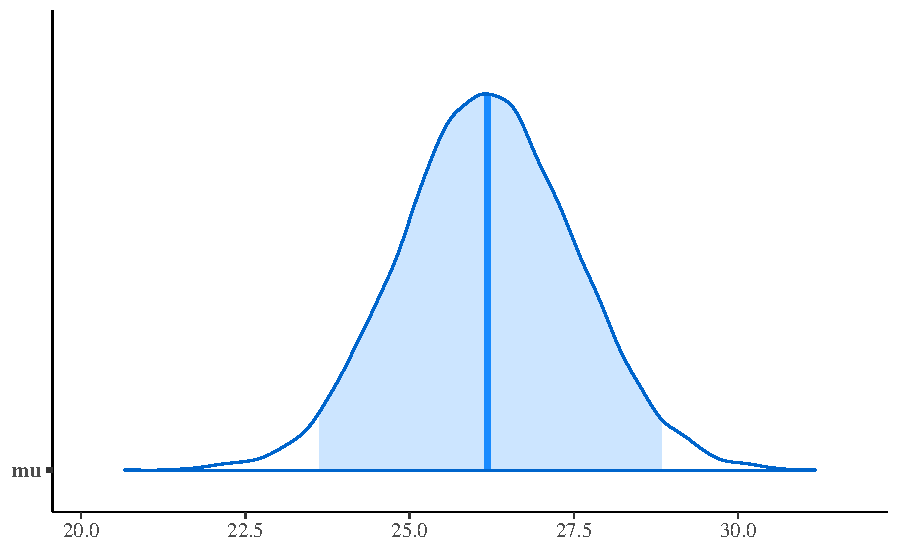
\includegraphics[width=0.8\linewidth]{928_R_tidyverse_files/figure-latex/unnamed-chunk-20-1} \end{center}

Coloriamo ora in maniera diversa i punti che rappresentano animali carnivori, erbivori, ecc.

\begin{Shaded}
\begin{Highlighting}[]
\NormalTok{p }\OtherTok{\textless{}{-}}\NormalTok{ msleep }\SpecialCharTok{\%\textgreater{}\%} 
  \FunctionTok{ggplot}\NormalTok{(}
    \FunctionTok{aes}\NormalTok{(}\AttributeTok{x =}\NormalTok{ bodywt, }\AttributeTok{y =}\NormalTok{ sleep\_total, }\AttributeTok{col =}\NormalTok{ vore)}
\NormalTok{  ) }\SpecialCharTok{+}
  \FunctionTok{geom\_point}\NormalTok{()}
\FunctionTok{print}\NormalTok{(p)}
\end{Highlighting}
\end{Shaded}

\begin{center}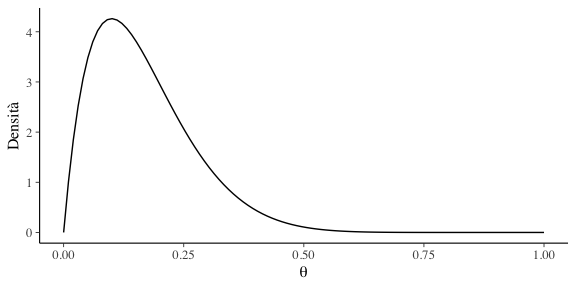
\includegraphics[width=0.8\linewidth]{928_R_tidyverse_files/figure-latex/unnamed-chunk-21-1} \end{center}

È chiaro, senza fare alcuna analisi statistica, che la relazione tra le due variabili non è lineare. Trasformando in maniera logaritmica i valori dell'asse \(x\) la relazione si linearizza.

\begin{Shaded}
\begin{Highlighting}[]
\NormalTok{p }\OtherTok{\textless{}{-}}\NormalTok{ msleep }\SpecialCharTok{\%\textgreater{}\%} 
  \FunctionTok{ggplot}\NormalTok{(}
    \FunctionTok{aes}\NormalTok{(}\AttributeTok{x =} \FunctionTok{log}\NormalTok{(bodywt), }\AttributeTok{y =}\NormalTok{ sleep\_total, }\AttributeTok{col =}\NormalTok{ vore)}
\NormalTok{  ) }\SpecialCharTok{+}
  \FunctionTok{geom\_point}\NormalTok{()}
\FunctionTok{print}\NormalTok{(p)}
\end{Highlighting}
\end{Shaded}

\begin{center}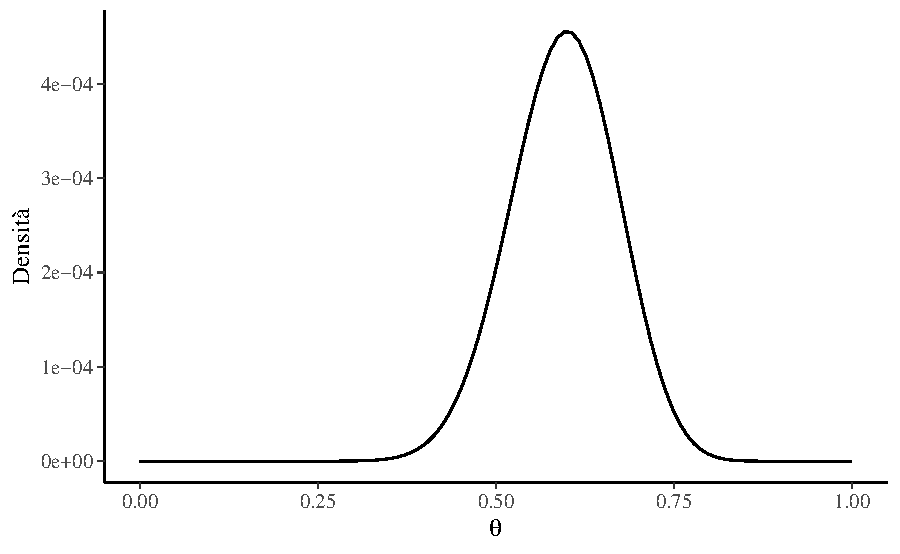
\includegraphics[width=0.8\linewidth]{928_R_tidyverse_files/figure-latex/unnamed-chunk-22-1} \end{center}

Infine, aggiustiamo il ``tema'' del grafico (si noti l'utilizzo di una tavolozza di colori adatta ai daltonici), aggiungiamo le etichette sugli assi e il titolo.

\begin{Shaded}
\begin{Highlighting}[]
\NormalTok{msleep }\SpecialCharTok{\%\textgreater{}\%}
  \FunctionTok{ggplot}\NormalTok{(}
    \FunctionTok{aes}\NormalTok{(}\AttributeTok{x =} \FunctionTok{log}\NormalTok{(bodywt), }\AttributeTok{y =}\NormalTok{ sleep\_total, }\AttributeTok{col =}\NormalTok{ vore)}
\NormalTok{  ) }\SpecialCharTok{+}
  \FunctionTok{geom\_point}\NormalTok{(}\AttributeTok{size =} \DecValTok{3}\NormalTok{) }\SpecialCharTok{+}
  \FunctionTok{scale\_color\_okabe\_ito}\NormalTok{(}\AttributeTok{name =} \StringTok{"vore"}\NormalTok{, }\AttributeTok{alpha =}\NormalTok{ .}\DecValTok{9}\NormalTok{) }\SpecialCharTok{+}
  \FunctionTok{theme}\NormalTok{(}\AttributeTok{legend.title =} \FunctionTok{element\_blank}\NormalTok{()) }\SpecialCharTok{+}
  \FunctionTok{labs}\NormalTok{(}
    \AttributeTok{x =} \StringTok{"Peso corporeo (log)"}\NormalTok{,}
    \AttributeTok{y =} \StringTok{"Ore di sonno"}\NormalTok{,}
    \AttributeTok{title =} \StringTok{"Il sonno in 83 specie di mammiferi"}\NormalTok{,}
    \AttributeTok{subtitle =} \StringTok{"Savage e West (2007)"}
\NormalTok{  )}
\end{Highlighting}
\end{Shaded}

\begin{center}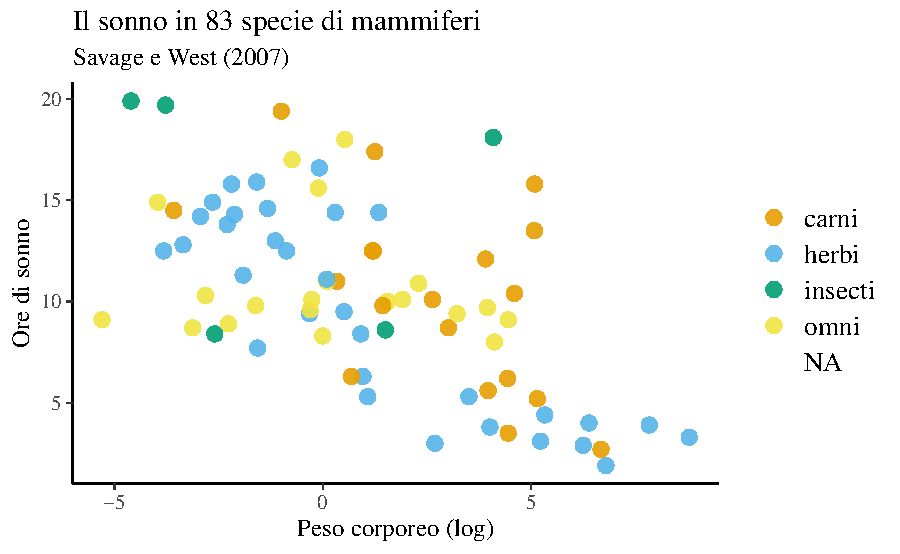
\includegraphics[width=0.8\linewidth]{928_R_tidyverse_files/figure-latex/unnamed-chunk-23-1} \end{center}

\hypertarget{istogramma}{%
\subsubsection{Istogramma}\label{istogramma}}

Creiamo ora un istogramma che rappresenta la distribuzione del (logaritmo del) peso medio del cervello delle 83 specie di mammiferi considerate da \textcite{savage2007quantitative}. L'argomento \texttt{aes(y\ =\ ..density..)} in \texttt{geom\_histogram()} produce le frequenze relative. L'opzione di default (senza questo argomento) porta \texttt{ggplot()} a rappresentare le frequenze assolute.

\begin{Shaded}
\begin{Highlighting}[]
\NormalTok{msleep }\SpecialCharTok{\%\textgreater{}\%} 
  \FunctionTok{ggplot}\NormalTok{(}
    \FunctionTok{aes}\NormalTok{(}\FunctionTok{log}\NormalTok{(brainwt))}
\NormalTok{  ) }\SpecialCharTok{+}
  \FunctionTok{geom\_histogram}\NormalTok{(}\FunctionTok{aes}\NormalTok{(}\AttributeTok{y =}\NormalTok{ ..density..)) }\SpecialCharTok{+}
  \FunctionTok{labs}\NormalTok{(}
    \AttributeTok{x =} \StringTok{"Peso del cervello (log)"}\NormalTok{,}
    \AttributeTok{y =} \StringTok{"Frequenza relativa"}
\NormalTok{  ) }\SpecialCharTok{+}
  \FunctionTok{theme}\NormalTok{(}\AttributeTok{legend.title =} \FunctionTok{element\_blank}\NormalTok{())}
\end{Highlighting}
\end{Shaded}

\begin{center}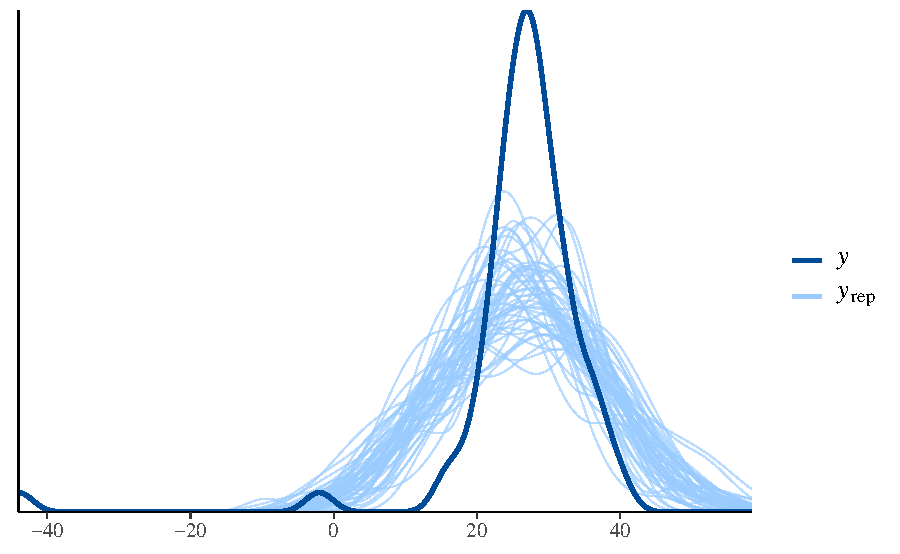
\includegraphics[width=0.8\linewidth]{928_R_tidyverse_files/figure-latex/unnamed-chunk-24-1} \end{center}

\hypertarget{scrivere-il-codice-in-r-con-stile}{%
\subsection{\texorpdfstring{Scrivere il codice in \texttt{R} con stile}{Scrivere il codice in R con stile}}\label{scrivere-il-codice-in-r-con-stile}}

Uno stile di programmazione è un insieme di regole per la gestione dell'indentazione dei blocchi di codice, per la creazione dei nomi dei file e delle variabili e per le convenzioni tipografiche che vengono usate. Scrivere il codice in \texttt{R} con stile consente di creare listati più leggibili e semplici da modificare, minimizza la possibilità di errore, e consente correzioni e modifiche più rapide. Vi sono molteplici stili di programmazione che possono essere utilizzati dall'utente, anche se è bene attenersi a quelle che sono le convenzioni maggiormente diffuse, allo scopo di favorire la comunicazione. In ogni caso, l'importante è di essere coerenti, ovvero di adottare le stesse convenzioni in tutte le parti del codice che si scrive. Ad esempio, se si sceglie di usare lo stile \texttt{snake\_case} per il nome composto di una variabile (es., \texttt{personality\_trait}), non è appropriato usare lo stile \emph{lower Camel case} per un'altra variabile (es., \texttt{socialStatus}). Dato che questo argomento è stato trattato ampiamente in varie sedi, mi limito qui a rimandare ad uno stile di programmazione molto popolare, quello proposto da Hadley Wickham, il creatore di \texttt{tidyverse}. Potete trovare maggiori informazioni al seguente link: \url{http://style.tidyverse.org/}.


% Bibliography
%%%%%%%%%%%%%%%%%%%%%%%%%%%%%%%%%%%%%%%%%%%%%%%%%%%%%%%%%%

\backmatter
\SmallMargins

\printbibliography
\onecolumn


% Tables (of tables, of figures)
%%%%%%%%%%%%%%%%%%%%%%%%%%%%%%%%%%%%%%%%%%%%%%%%%%%%%%%%%%


\cleardoublepage
\LargeMargins
\listoffigures


% After-body (LaTeX code inclusion)
%%%%%%%%%%%%%%%%%%%%%%%%%%%%%%%%%%%%%%%%%%%%%%%%%%%%%%%%%%




% Back cover
%%%%%%%%%%%%%%%%%%%%%%%%%%%%%%%%%%%%%%%%%%%%%%%%%%%%%%%%%%%

% Even page, small margins, no running head, no page number.
\evenpage
\SmallMargins
\thispagestyle{empty}

\begin{normalsize}

\begin{description}

\selectlanguage{italian}
\item[Abstract]
This document contains the material of the lessons of Psicometria B000286 (2021/2022) aimed at students of the first year of the Degree Course in Psychological Sciences and Techniques of the University of Florence, Italy.
\item[Keywords]
Data science, Bayesian statistics.
~\\

\end{description}

\end{normalsize}


\end{document}
